\documentclass[12pt,a4paper]{scrartcl}
\author{Lecture: Martin Hering-Betram}
\usepackage[english]{babel}
\usepackage[none]{hyphenat}
\usepackage[T1]{fontenc}
\usepackage{graphicx, subfig}
\graphicspath{{img/}}
\usepackage[document]{ragged2e}
\usepackage{lmodern}
\usepackage{color}
\usepackage{amsmath}
\usepackage{graphicx}
 
\title{Documentation - Computer Graphics Project 1}
\date{24. April 2018}

\begin{document}


\maketitle

\begin{center}

\Large
\textbf{Field of study:} Media informatics
\\
\textbf{Semester:} 4
\\[3cm]
\textbf {Authors:}
\\Fabian Niehaus
\\501297
\\Tuyet Nguyen
\\5009445

\end{center}
\newpage
\Large
\tableofcontents
\newpage
\Large
\vspace{3cm}


\section{Abstract}
In this project we will build a C++ application that can read, render and write quad meshes as well as apply the Catmull-Clark subdivision algorithm. We will use QT Creator for programming, QT for window management and OpenGL for 3D rendering.

\section{Realisation}

\subsection{Creating the data structure}
In the first step, the data structure for storing vertices and quads is implemented. This structure consist of a class "Vertex" containing the three coordinates and the valence and a class "Quad" containing the indices of four vertices, the indices of four adjacent quads, the index of its face vertex and the four indices of its edge vertices, the latter two being calculated in the process of the Catmull-Clark subdivision. The individual vertices and quads are stored in a vector list each.

\subsection{Reading the data from a file}
After creating the required data structure, a method for reading the vertices and faces from an .obj file is implemented. For this project we can assume that every face is a quad. The distinction between a vertex and a quad is made by the first letter in the line, a "v" for vertices and an "f" for quads. //
Each line is read, and depending on the first letter a new Vertex or Quad is created and pushed to the respective vector.
If everything has been read correctly, a "true" value is returned.

\subsection{Rendering}
In order to render the quads, a new class inheriting QTs QOpenGLWidget is implemented. This class, called OGLWidget, needs to implement the following methods: initializeGL (for setting up OpenGL), paintGL (for doing the actual rendering), resizeGL (for handling resizes of the display window). Additionally, the functions SetMaterialColor and InitLightingAndProjection are implemented.

\subsubsection{Rendering as GL_LINES}

\large
\textbf{Problem} \\
-Develop a class Vertex and a class Quad. The Vertex class may contain three coordinates and the
valence (number of edges). The Quad class may contain the indices of four vertices and of four
adjacent quads. Normal vectors can be calculated from the cross product between two diagonals.\\
-Implement a function to read points and faces from OBJ. You can assume that all faces are quads (for an example, see cube.obj). Since the number of vertices and quads is not known before reading the file, static arrays are not a good choice. Instead, vectors may be used: vector vertices; vector quads;\\
-Implement a function drawing the mesh c1 as quadrilateral polygons and c2 as wireframe, using GLQUADS (with normal vectors and lighting) and GLLINES (without lighting), respectively.\\[0,5cm]

In order to render Quads Meshes read from an .obj file, we need a data structure to store vertices and quads. The vertices need to contain their three coordinates as well their valence. The quads need to store their four corner vertices and their four adjacent quads.
To fill the data structure with actual data, a method that reads the .obj file ist required. We can assume that every face is a quad.
Lastly a rendering environment is needed. We will render the object twice - once as a simple wireframe without lighting and once as a solid cube with lighting.


\textbf{Approach}\\
As a framework for solving the problem we used OpenGL and QT Creator. In the program QT the Vertex class and Quad class are created.\\

We use QTCreator with OpenGL for window management and 3D rendering for this as well as all following problems.

A vertex class with three intergers for coordinates as well as an integer for the valence is implemented.
Then, a quad class with four integers for the vertex indices and four integers for the 

The vertex class contains the information of three x,y,z coordinates and the valence. In the Quads class has the four edges vertices and of four adjacent.\\
For the next task, the points and faces are to be read from the file Cube.obj with the help of the "pushback" method. The file Cube is predefined. \\
Two squares are created for the last task. There are quadrilateral polygons and as wireframe..The oglwidget and oglwidget2 class are defined here.There two can be showed on diffirent windows. This step can be done with mainwindown.ui.\\
We used a "for" loop here. The methods in "for" loop read the points and connect the points with the lines(polygons) .And we used the same methos for the 3D Object (wireframe)\\[0,5cm]

\newpage

\textbf{Implementation}\\


Vertex define --> vertex.cpp\\
Quad define --> quad.cpp\\
read points and faces --> oglwidget2.cpp / line 3\\
draw quad --> oglwidget2.cpp / line 37 to 64\\
draw 3D-quad --> oglwidget2.cpp / line 72 to 90\\
SetMaterialColor --> oglwidget2.cpp / line 109 to 132\\
InitLightingAndProjection --> oglwidget2.cpp / line 133 to 166\\
initializeGL() --> line 167 to 183\\
paintGL --> line 185 to 210\\
resizeGL --> line 212 to 216 \\[0,5cm]



\textbf{Result}\\

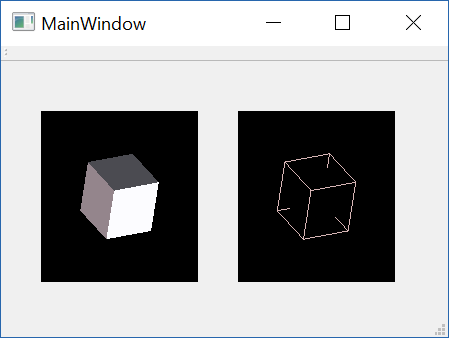
\includegraphics[width=0.7\textwidth]{Problem 1.png}\\

\subsection{Problem 2: Mesh Connectivity}

\large
\textbf{Problem}\\
-Implement a function calculating the vertex valences and connecting each quad to its neighbors.
You can assume that the mesh does not have boundaries, i.e. every quad has four neighbors.\\
-Print the entire data structure on the screen (or into a file). Devise and perform tests to validate
its correctness.\\
The mesh connectivity provides the basis for Catmull-Clark subdivision, which will be subject of the
next assignment.\\[0,5cm]

\textbf{Approach}\\
We have taken the following steps in this task.\\
+) We have a method to count the edge.\\
+) Then a method was created to search for the edge neighbours. The method takes a square and then looks for each of the 4 edges of this square, if any other square divides this edge, respectively these 2 corner points.\\[0,5cm]

\textbf{Implementation}\\
calculateVertexValence--> oglwidget.cpp / line 109 to 139\\
compareVertices --> vertex.cpp / line 51 to 61\\
determineQuadNeighbours --> oglwidget.cpp / line 143 to 178\\[0,5cm]

\textbf{Results}\\


\newpage

\section{Excercise 2}

\subsection{Problem 1: Catmull-Clack Subdivision Masks}

\large
\textbf{Problem}\\
- Implement the face subdivision mask (f = durchschnitt von v(f)) computing the midpoint of each quad and adding it to the vertex vector\\
- Based on the mesh connectivity structure from exercise 1, find a way to computer and add the edge vertices to the vertex vector\\
- Implement the vertex mask, modifying the original vertices\\
 
\textbf{Approach}\\
\textbf{Implementation}\\
\textbf{Results}\\
\subsection{Problem 2: Recursive Subdivision}

\large
\textbf{Problem}\\
Replace every face by the four sub-faces connected to the correct vertices. Restore the mesh
connectivity and apply two more subdivisions before rendering. \\
\textbf{Approach}\\
The method subdivideAndReconnectMesh is provided. The function builds a square of one point with two its edge point and one face point.\\
\textbf{Implementation}\\
subdivideAndReconnectMesh --> oglwidget /Line 256 to 280\\
\textbf{Results}\\

\end{document}
